\subsubsection{\stid{4.14} ECP EZ: Fast, Effective, Parallel Error-bounded Exascale Lossy Compression for Scientific Data}

\paragraph{Overview}

Extreme scale simulations and experiments are generating more data than can be stored, communicated and analyzed. Current lossless compression methods suffer from low compression ratio and do not adequately address the limitations in storage bandwidth and storage space of projected exascale systems. Existing lossy compressors, although enabling greater data reduction, are not covering the needs of many ECP applications.

The EZ project is extending and improving the SZ lossy compressor for structured and unstructured scientific datasets respecting user-set error controls. SZ offers an excellent compression ratio and compression time. Further work is essential, however, to improve our SZ lossy compressor for ECP scientific datasets, while ensuring that user-set error controls are respected. Specifically, we are maximizing the effectiveness of SZ’s three core compression algorithms: prediction, quantization, and coding. The EZ project focuses on optimization of the compression quality, including improvement of compression ratio, memory cost minimization, parallelization, addition of more error controls, and integration of SZ into parallel I/O environments (PnetCDF, ADIOS, HDF5). Our goal is to produce a high-quality lossy compressor responding to the needs of ECP exascale applications and experiment users. To this end, we are working with multiple ECP application teams, including ExaSky cosmology teams (HACC and Nyx), molecular dynamics simulations groups (EXAALT), x-ray laser imaging experimentalists (ExaFEL), and computational chemists (NWChem-X, GAMESS) to optimize SZ for their applications and to harden SZ for production use.

\paragraph{Key Challenges}

There are several key challenges in the EZ project.
\begin{itemize}
\item One challenge in designing an efficient compressor for HPC applications is the large
diversity of scientific data, such as various dimensions, scales, and dynamic data changes in both
space and time.
\item Another challenge is that the scientific data may have irregular characteristics. The simulation data may exhibit spiky changes in small regions. For instance, the data in HACC simulation are all stored in 1D arrays: three coordinate fields (xx, yy, zz) and three velocity fields (vx, vy, vz). It is hard to get a high compression ratio because of lack of correlations between adjacent particles in each array.
\item It is non trivial to support random access under the traditional SZ compression model, which has a relatively strong dependency among the data points during the compression/decompression. 
\item Integrating SZ into parallel I/O libraries (such as PnetCDF and HDF5) is non-trivial, because these I/O libraries are designed and implemented differently with various interfaces. We need to develop the integration codes carefully based on the I/O libraries' interface with minimal cost.
\item It is non-trivial to parallelize SZ to get a high speed-up. A new version (SZ 2.0) (released on July 26th) significantly improved the compression quality for high-compression cases, but also introduced more challenges on the implementation of parallel version of SZ. Specifically, SZ 2.0 splits the whole dataset into multiple non-overlapped small blocks (such as 8x8x8) and performs the compression in each block by selecting an adaptive prediction method. SZ 2.0 still has a certain dependency across the blocks in the block-wise compression, which is a challenge for the implementation over GPU. 

\end{itemize}

\paragraph{Solution Strategy}

As for the first challenge, we keep a close communication with ECP application users to understand their specific demands on the lossy compression. For instance, we have a weekly meeting with ECPSky team to discuss the required error bounds and compression quality of cosmology simulation data. We also provide multiple types of error bounds (such as absolute error bound, PSNR, relative error bound) allowing users to control the errors in different ways. We also exploit an adaptive prediction method to optimize the compression quality for diverse datasets. 

As for the second challenge, we develop some particular compression techniques based on specific data features across different applications.

As for the third challenge, we split each dataset into multiple non-overlapped small blocks and ensure that the compression in each block is totally independent with other blocks. To this end, we reorganize the data access in the code and separating the Huffman encoding function. 

We overcome the last challenge by understanding the principle of the I/O libraries deeply (either reading the related documents carefully or communicating with the I/O library developers closely).

As for the fourth challenge, the work is still under the progress. We will develop the GPU version of SZ based on the random-access support code, and explore some new compression techniques (such as replacing Huffman encoding by arithmetic encoding) if necessary.  

\paragraph{Recent Progress}

SZ 2.0 is released as an open source on github. Figure \ref{fig:sz-principle} (a) demonstrates the core step (data prediction and linear-scaling quantization) in SZ lossy compression using a 2D dataset. Figure \ref{fig:sz-principle} (b) demonstrates the visual quality of decompressed data for ECPSky-NYX VX field: SZ 2.0 has a pretty high visual quality with a high compression ratio of 156:1. This paper was accepted by IEEE BigData18.

\begin{figure}[htb]
\centering
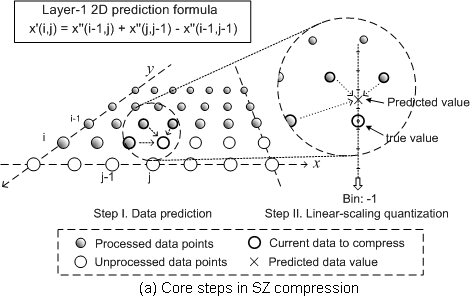
\includegraphics[width=2.8in]{projects/2.3.4-DataViz/2.3.4.14-VeloC-SZ/sz-illu.png}
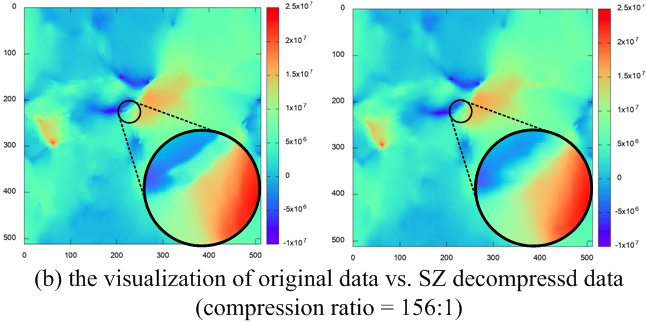
\includegraphics[width=3.2in]{projects/2.3.4-DataViz/2.3.4.14-VeloC-SZ/Visual-quality-NYX-SZ.png}
\vspace{-2mm}
	\caption{\label{fig:sz-principle}Illustration of data prediction in SZ and visual quality of decompressed data for ECPSky-NYX VX field}
\end{figure}

We have improved the compression quality for some ECP applications significantly. For instance, we develop PaSTRI code that can significantly improve the compression ratio for GAMESS two-electron integral datasets by leveraging the potential scaled repeated patterns, and this work is awarded as the overall best paper in IEEE CLUSTER18. We also implemented effective compression method supporting point-wise relative error bounds for the ECPSky project and studied its lossy compression quality with multiple resolutions. Experiments with point-wise relative error bound based compression shows that our solution leads to 31\%-210\% higher compression ratio than other lossy compressors do. It also receives the best-paper award in the software track of IEEE CLUSTER18. We completed the integration of SZ into different I/O libraries such as HDF5 and ADIOS. 

We also improved compression quality for cosmological simulation by developing an in-situ time-dimension based compression mechanism. From Fig. \ref{fig:szcompression} (a), we see that our solution (labeled as SZ\_vlct) exhibits much better rate-distortions than others. Fig. \ref{fig:szcompression} (b) shows the break-down of the data dumping/loading times of three solution (SZ\_single\_snapshot, SZ\_prestep, and SZ\_vlct). We can see that our solution leads to the shortest overall I/O time. We present the random-access performance evaluation results in Fig. \ref{fig:szcompression} (c), which shows that the random-access function in SZ 2.0 can significantly reduce the decompression time on demand. 

\begin{figure}[htb]
\centering
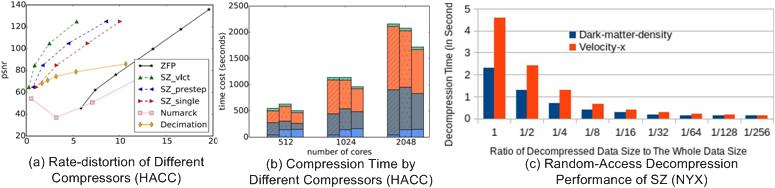
\includegraphics[width=6in]{projects/2.3.4-DataViz/2.3.4.14-VeloC-SZ/time-based-comp-and-random.jpg}
\vspace{-2mm}
\caption{Compression Results of Time-based SZ and Random-Access}
\label{fig:szcompression}
\vspace{-5mm}
\end{figure}

\paragraph{Next Steps} Our next efforts are: Improve compression performance by analyzing SZ's performance and implementing the parallel version over GPU.

%\textbf{Support advanced error controls allowing the user to specify relative error bounds and to control the error distribution.} We will write a report describing the integration of additional error controls (relative error bound and control of error distribution) in SZ.
